\chapter{Antiderivatives}

In your study of calculus, you have learned about derivatives, which
allow us to find the rate of change of a function at any given
point. Derivatives are powerful tools that help us analyze the
behavior of functions. Now, we will explore another concept called
antiderivatives, which are closely related to derivatives.\index{Antiderivatives}

An antiderivative, also known as an integral or primitive, is the
reverse process of differentiation. It involves finding a function
whose derivative is equal to a given function. In simple terms, if you
have a function and you want to find another function that, when
differentiated, gives you the original function back, you are looking
for its antiderivative.

The symbol used to represent an antiderivative is $\int$. It is called
the integral sign. For example, if $f(x)$ is a function, then the
antiderivative of $f(x)$ with respect to $x$ is denoted as $\int f(x)
, dx$. The $dx$ at the end indicates that we are integrating with
respect to $x$.

Finding antiderivatives requires using specific techniques and
rules. Some common antiderivative rules include:

\begin{itemize}
\item The power rule: If $f(x) = x^n$, where $n$ is any real number
  except $-1$, then the antiderivative of $f(x)$ is given by $\int
  f(x) , dx = \frac{1}{n+1}x^{n+1} + C$, where $C$ is the constant of
  integration.

\item The constant rule: The antiderivative of a constant function is
  equal to the constant times $x$. For example, if $f(x) = 5$, then
  $\int f(x) , dx = 5x + C$.

\item The sum and difference rule: If $f(x)$ and $g(x)$ are functions,
  then $\int (f(x) + g(x)) , dx = \int f(x) , dx + \int g(x) ,
  dx$. Similarly, $\int (f(x) - g(x)) , dx = \int f(x) , dx - \int
  g(x) , dx$.
\end{itemize}

Antiderivatives have various applications in mathematics and
science. They allow us to calculate the total accumulation of a
quantity over a given interval, compute areas under curves, and solve
differential equations, among other things.

It is important to note that an antiderivative is not a unique
function. Since the derivative of a constant is zero, any constant
added to an antiderivative will still be an antiderivative of the
original function. This is why we include the constant of integration,
denoted by $C$, in the antiderivative expression.

A concrete example of this is $f(x) = x^2$. Let us define $F(x)$ such that $F'(x) = f(x)$. That is, there is some function $F$ such that the derivative of $F$ is $f$. One possible solution for $F$ is $F(x) = \frac{1}{3}x^3$. You can check using the power rule that $\frac{d}{dx}F(x) = f(x)$. What if we added or subtracted a constant from $F$? Let us define $G(x) = \frac{1}{3}x^3+2$. Well, $G'(x) = f(x)$ also! Same for $H(x) = \frac{1}{3}x^3-7$. Several possible antiderivatives of $f(x) = x^2$ are shown in figure \ref{fig:antideriv}. 

\begin{figure}
	\centering
	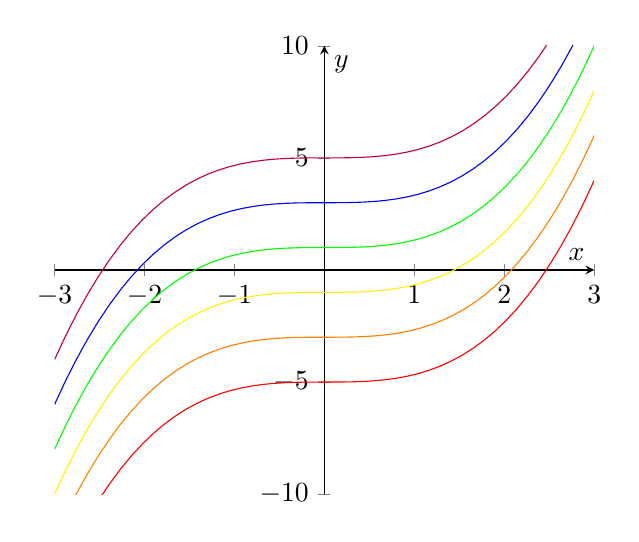
\begin{tikzpicture}
		\begin{axis}[xmin=-3, xmax=3, axis lines = center, xlabel=$x$, ylabel=$y$, ymin=-10, ymax=10]
		\addplot[red, samples=50, domain=-3:3]{(1/3)*x^3 - 5};
		\addplot[orange, samples=50, domain=-3:3]{(1/3)*x^3 - 3};
		\addplot[yellow, samples=50, domain=-3:3]{(1/3)*x^3 - 1};
		\addplot[green, samples=50, domain=-3:3]{(1/3)*x^3 + 1};
		\addplot[blue, samples=50, domain=-3:3]{(1/3)*x^3 +3};
		\addplot[purple, samples=50, domain=-3:3]{(1/3)*x^3 + 5};
		\end{axis}
	\end{tikzpicture}
	\caption{Several possible solutions to $F'(x) = x^2$}
	\label{fig:antideriv}
\end{figure} 

Since taking a derivative "erases" any constant, you must always add back in the unknown constant, $C$, when finding the general antiderivative. If you are given a condition, you can often solve for $C$ and find a specific antiderivative. For example, suppose that in addition to knowing that $F'(x) = x^2$, we also know that $F(3) = 2$. We can use the fact that $F$ passes through $(3, 2)$ to find the value of $C$:

$$F(x) = \frac{1}{3}x^3+C$$
$$F(3) = \frac{1}{3}(3)^2+C = 2$$
$$39+C=2$$
$$C=-7$$

Therefore, the specific solution to $F'(x) = x^2$ with the condition that $F(3) =2$ is $F(x) = \frac{1}{3}x^3-7$. 

\begin{Exercise}[label=antideriv1]
	A particle moving in a straight line has an acceleration given by $a(t) = 6t+4$. If its initial velocity is $-6 \frac{cm}{s}$ and its initial position is $9 cm$, what is the function $s(t)$ that describes the particle's position?
\end{Exercise}

\begin{Answer}[ref=antideriv1]
	First, we will find $v(t)$ by taking the antiderivative of $a(t)$ and using the initial condition $v(0) = -6$
	$$\int 6t+4\,dt = 3t^2+4t+C=v(t)$$
	$$v(0) = 3(0)^2+4(0)+C=-6$$
	$$C = -6$$
	Therefore, the velocity function is $v(t) = 3t^2+4t-6$. Now we repeat the process to find $s(t)$:
	$$\int 3t^2+4t-6 \,dt = t^3+2t^2-6t+C=s(t)$$
	$$s(0) = (0)^3+2(0)^2-6(0)+C = 9$$
	$$C=9$$
	Therefore, the position function is $s(t) = t^3+2t^2-6t+9$. 
\end{Answer}

\begin{Exercise}[label=antideriv2]
	Let $f'(x) = 2\sin{x}$. If $f(\pi) = 1$, write an expression for $f(x)$. 
\end{Exercise}

\begin{Answer}[ref=antideriv2]
	The antiderivative of $\sin{x}$ is $-\cos{x}$ and therefore the general solution is $f(x) = -2\cos{x}+C$. We use the given condition, $f(\pi) = 1$ to find $C$:
	$$f(\pi) = -2\cos{\pi}+C = 1$$
	$$C = 1+2\cos{\pi}=1+2(-1) = -1$$
	Therefore, the specific solution is $f(x) = -2\cos{x}-1$
\end{Answer}

\begin{Exercise}[label=antideriv3]
		
\end{Exercise}

\begin{Answer}[ref=antideriv3]
	
\end{Answer}

In summary, antiderivatives are the reverse process of
differentiation. They help us find functions whose derivatives match a
given function. Understanding antiderivatives is crucial for various
advanced calculus concepts and real-world applications.

Now, let's explore different techniques and methods for finding
antiderivatives and discover how they can be applied in solving
problems.

